



trim={<left> <lower> <right> <upper>}
























		\begin{itemize}
			\item Web document clustering (ZAMIR; ETZIONI, 1998); 
			\item Multi-topic multi-document summarization  (MASAO; KôITI, 2000); 
			\item Multi-document topic segmentation (JEONG; TITOV, 2010); 
			\item A Study on Statistical Generation of a Hierarchical Structure of Topic-information for Multi-documents (NGUYEN, 2011); 
			\item A segment-based approach to clustering multi-topic documents (TAGARELLI; KARYPIS, 2013).

		\end{itemize}








  \begin{center}
	\begin{figure}[h!]

	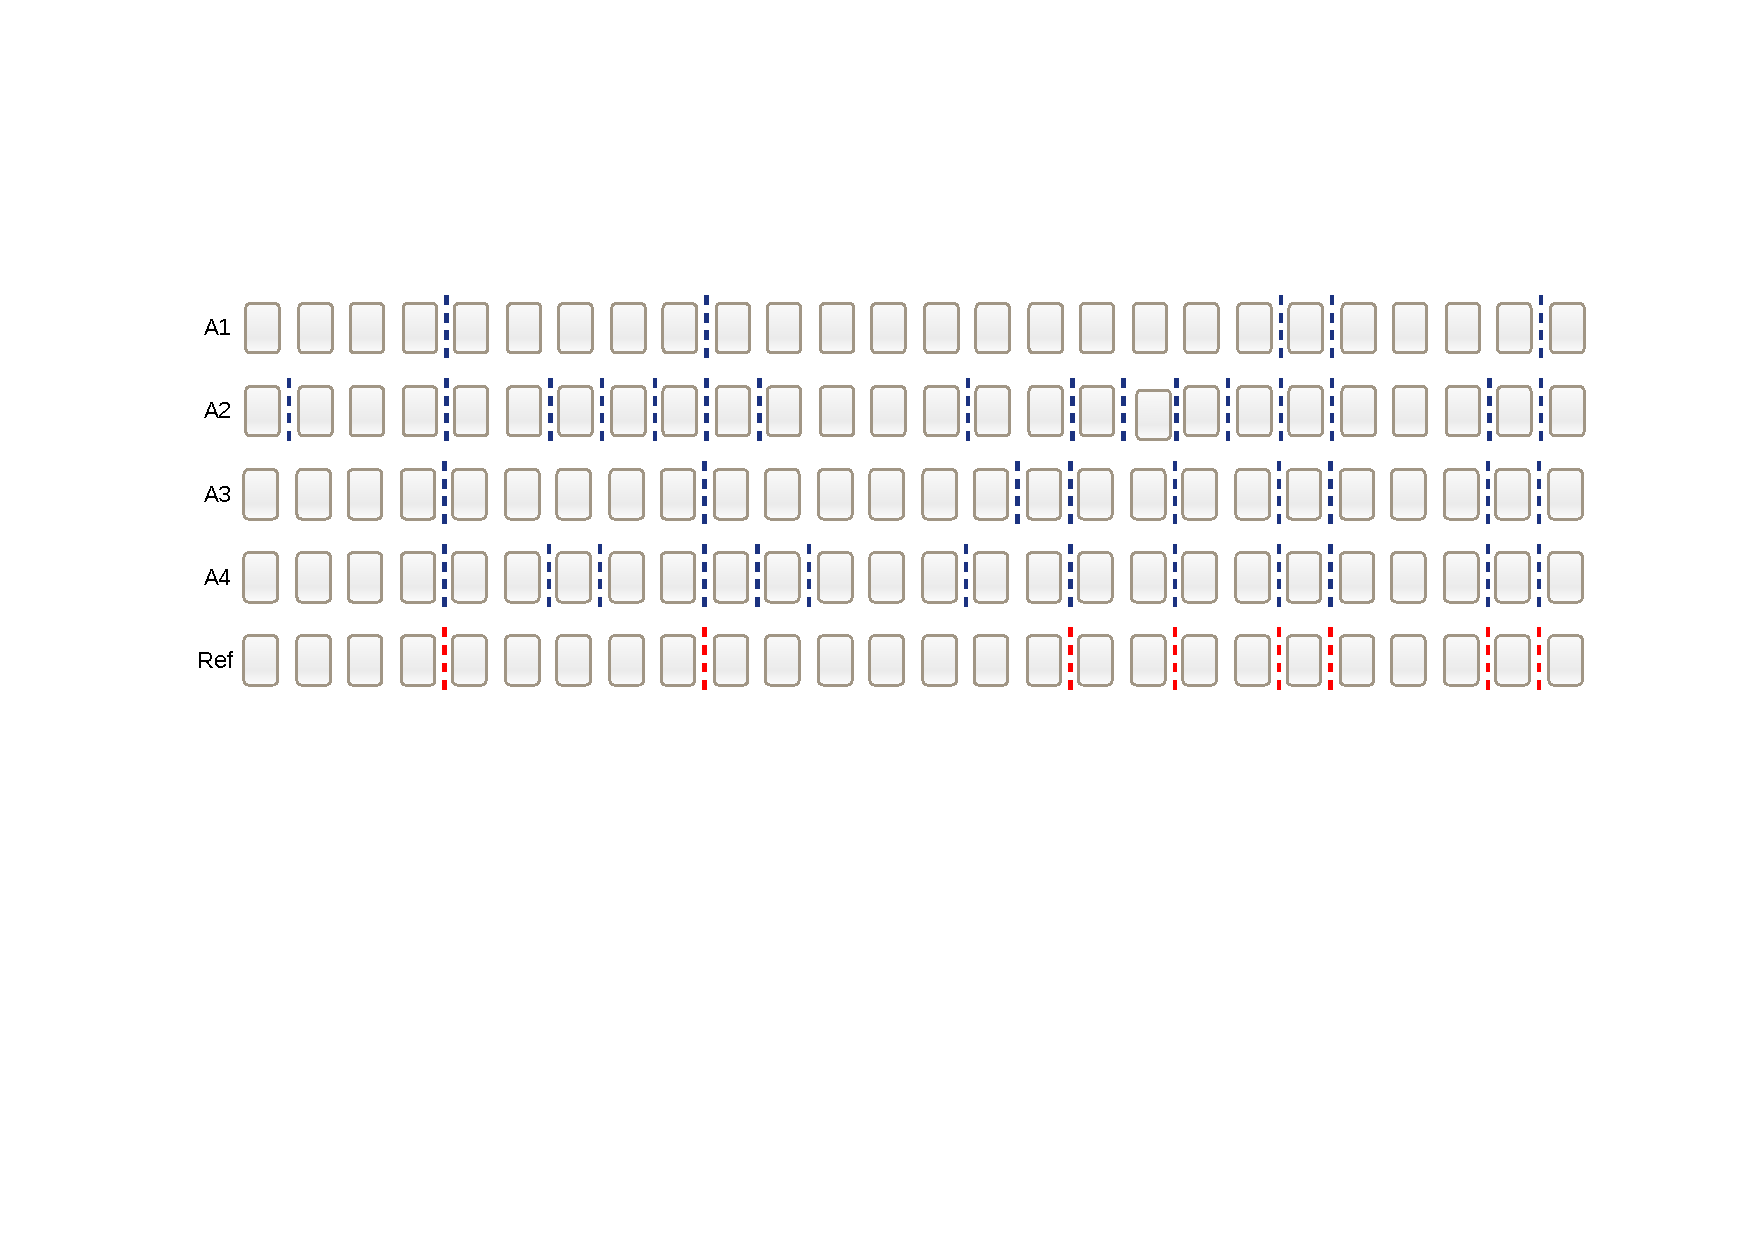
\includegraphics[trim={ 95 255 75 140 },clip,page=1,width=\textwidth]{images/segmentacao-referencia.pdf}

	% \caption{Exemplo uma segmentação de referência criada a partir da concordância entre segmentações manuais.}
	\end{figure}
\end{center}











\begin{table}[!h]
	\centering
	\begin{tabular}{|l|c|c|c|c|c|c|c|c|c|c|c|c|c|} \hline
		\textbf{Ata} & \textbf{\#Sent.}  & 
		\textbf{A1}  & 
		\textbf{A2}  & 
		\textbf{A3}  & 
		\textbf{A4}  & 
		\textbf{A5}  & 
		\textbf{A6}  & 
		\textbf{A7}  & 
		\textbf{A8}  & 
		\textbf{A9} 
		\\	\hline
% 		              A1   A2   A3  A4    A5   A6   A7   A8   A9   
		Ata 1  & 25 & 7  & 4  & 11 & 6  & 16 & 8  & 8  & 15 & 16 \\ \hline 
		Ata 2  & 17 & 4  & 4  & 8  & 6  & 11 & 6  & 6  & 15 & 14 \\ \hline 
		Ata 3  & 26 & 6  & 6  & 8  & 4  & 15 & 9  & 10 & 18 & 14 \\ \hline 
		Ata 4  & 26 & 5  & 5  & 10 & 6  & 14 & 17 & 7  & 11 & 12 \\ \hline 
		Ata 5  & 33 & 4  & 4  & 6  & 5  & 17 & 22 & 9  & 18 & 16 \\ \hline 
		Ata 6  & 11 & 3  & 4  & 6  & 4  & 9  & 9  & 4  & 7  &  5 \\ \hline 
		Ata 7  & 20 & 3  & 7  & 5  & 4  & 11 & 14 & 5  & 5  &  4 \\ \hline 
		Ata 8  & 35 & 4  & 8  & 3  & 8  & 12 & 17 & 5  & 11 &  9 \\ \hline 
		Ata 9  & 24 & 3  & 5  & 3  & 6  & 11 & 11 & 3  & 9  &  9 \\ \hline 
		Ata 10 & 50 & 4  & 5  & 4  & 7  & 31 & 29 & 5  & 9  &  8 \\ \hline 
		Ata 11 & 43 & 4  & 7  & 5  & 7  & 29 & 19 & 5  & 9  & 12 \\ \hline 
		Ata 12 & 56 & 3  & 10 & 4  & 16 & 33 & 25 & 4  & 13 & 11 \\ \hline 
		\textbf{Total} &
		\textbf{366} & 
		\textbf{50}&  
		\textbf{69} & 
		\textbf{73}&  
		\textbf{79}&  
		\textbf{209} & 
		\textbf{186}&  
		\textbf{71}&  
		\textbf{140}&  
		\textbf{130} 
		\\ \hline 

	\end{tabular}
	\caption{Descrição dos resultados obtidos com anotadores. Na segunda coluna \#Sent., é mostrada a quantidade de sentenças de cada ata. Nas colunas A1-A9 é mostrado as quantidades de segmentos informados pelos anotadores. 
	% As colunas K, P$_k$ e WD indicam respectivamente as médias de \textit{Kappa}, $P_k$ e \textit{WindowDiff}.
} 

	\label{tab:ataseanotacoes}
\end{table}

















\begin{figure}[!h] \centering     %%% not \center

		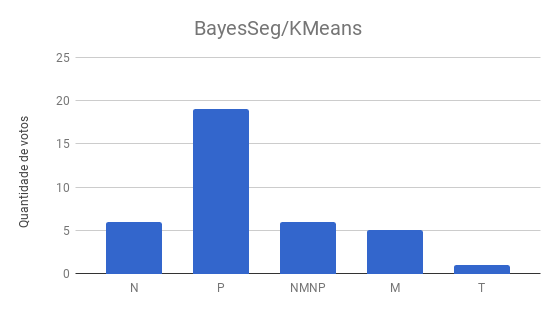
\includegraphics[width=.31\textwidth]{images/figuras-experimento/t1q3.png}
		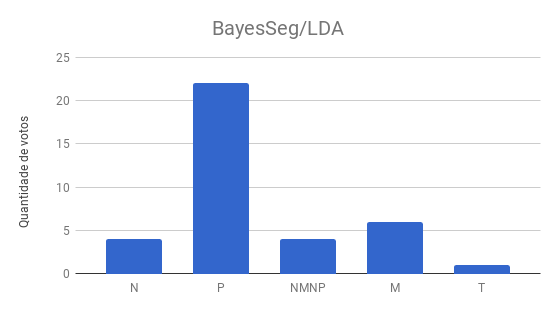
\includegraphics[width=.31\textwidth]{images/figuras-experimento/t2q3.png}
		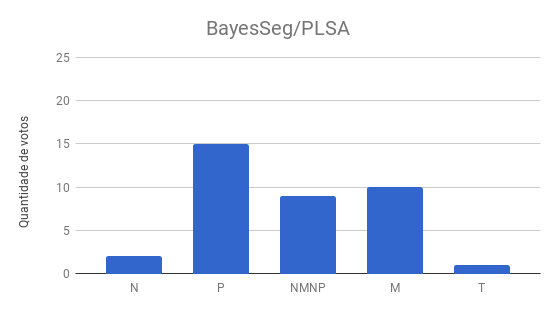
\includegraphics[width=.31\textwidth]{images/figuras-experimento/t3q3.png}

	% \caption{Contagem das respostas referentes a terceira questão, isolando-se as técnicas de extração de tópicos.}
	\label{fig:influenciaExtSegQ3}
\end{figure}


\begin{figure}[!h] \centering     %%% not \center

		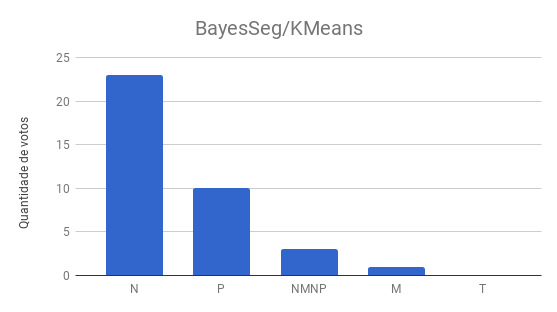
\includegraphics[width=.31\textwidth]{images/figuras-experimento/t1q4.png}
		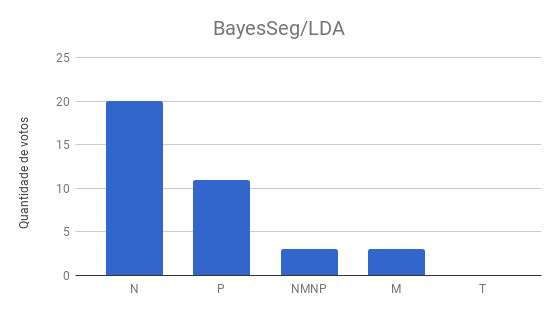
\includegraphics[width=.31\textwidth]{images/figuras-experimento/t2q4.png}
		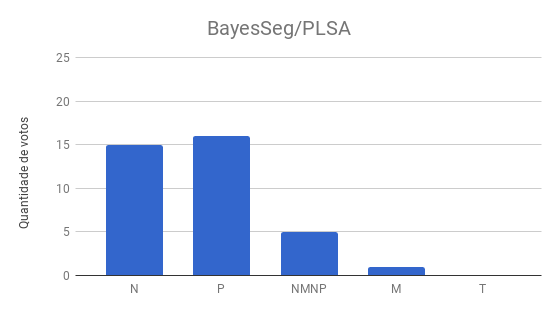
\includegraphics[width=.31\textwidth]{images/figuras-experimento/t3q4.png}

	% \caption{Contagem das respostas referentes a quarta questão, isolando-se as técnicas de extração de tópicos.}
	\label{fig:influenciaExtSegQ4}
\end{figure}






Primeira questão:\textit{``Todos os trechos apresentados compartilham um mesmo assunto.''}. 


	Segunda questão:\textit{``As palavras \textit{$<$descritores$>$} resumem bem o assunto tratado nos trechos.''}.


	Terceira questão:\textit{``Existem trechos que não tratam de um único assunto?''}. 
	
	Quarta questão:\textit{``Existem trechos incompletos e insuficientes para compreensão do assunto do trecho?''}.

\begin{figure}[!h] \centering     %%% not \center

		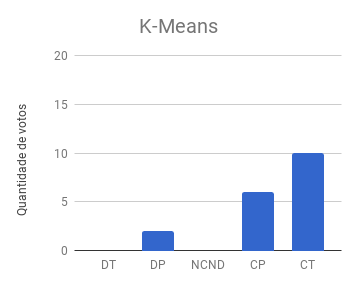
\includegraphics[width=.31\textwidth]{images/figuras-experimento/C1-Q1-KMeans.png}
		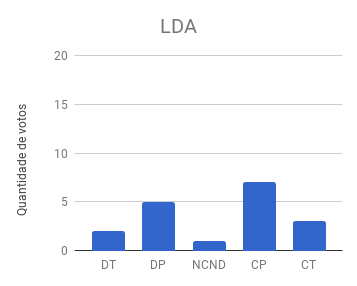
\includegraphics[width=.31\textwidth]{images/figuras-experimento/C1-Q1-LDA.png}
		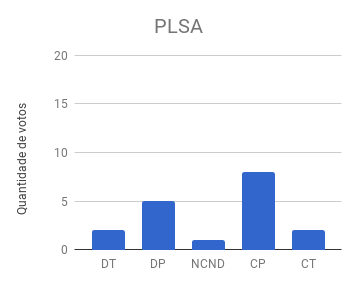
\includegraphics[width=.31\textwidth]{images/figuras-experimento/C1-Q1-PLSA.png}
		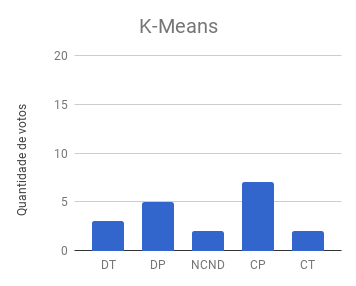
\includegraphics[width=.31\textwidth]{images/figuras-experimento/C2-Q1-KMeans.png}
		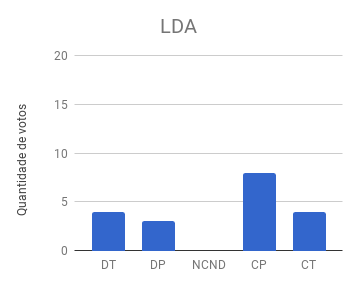
\includegraphics[width=.31\textwidth]{images/figuras-experimento/C2-Q1-LDA.png}
		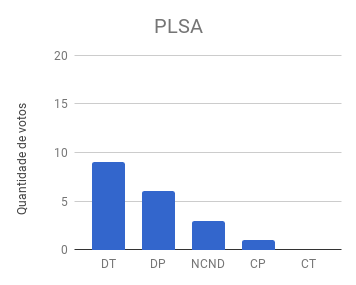
\includegraphics[width=.31\textwidth]{images/figuras-experimento/C2-Q1-PLSA.png}

	% \caption{Contagem das respostas referentes a Primeira questão. A primeira consulta, ``\textit{compra de equipamentos}'', é mostrada na linha superior e a segunda consulta, ``\textit{defesa de dissertação}'', na linha inferior.}
\end{figure}




\begin{figure}[!h] \centering     %%% not \center

		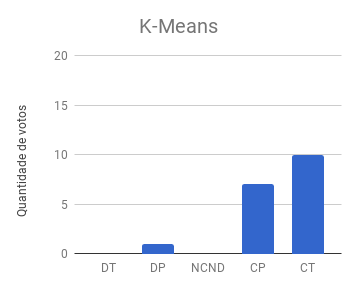
\includegraphics[width=.31\textwidth]{images/figuras-experimento/C1-Q2-KMeans.png}
		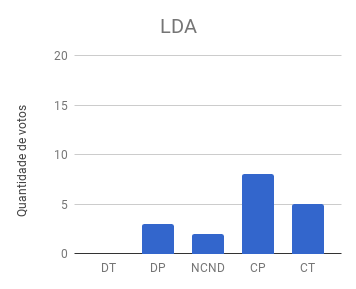
\includegraphics[width=.31\textwidth]{images/figuras-experimento/C1-Q2-LDA.png}
		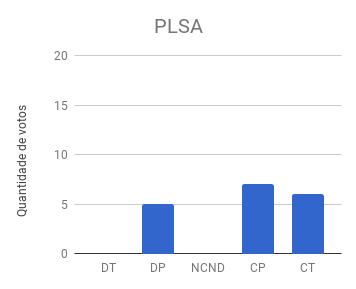
\includegraphics[width=.31\textwidth]{images/figuras-experimento/C1-Q2-PLSA.png}
		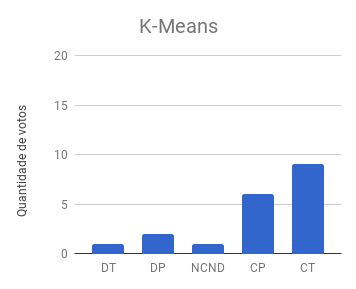
\includegraphics[width=.31\textwidth]{images/figuras-experimento/C2-Q2-KMeans.png}
		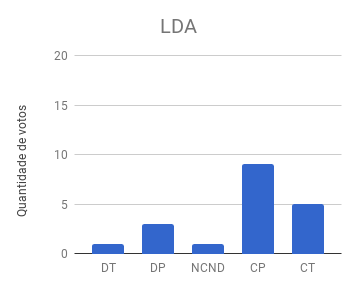
\includegraphics[width=.31\textwidth]{images/figuras-experimento/C2-Q2-LDA.png}
		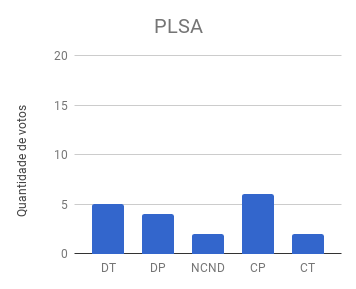
\includegraphics[width=.31\textwidth]{images/figuras-experimento/C2-Q2-PLSA.png}

	% \caption{Contagem das respostas referentes a Segunda questão. A primeira consulta, ``\textit{compra de equipamentos}'', é mostrada na linha superior e a segunda consulta, ``\textit{defesa de dissertação}'', na linha inferior.}
	\label{fig:c12-q2}
\end{figure}











\begin{table}
\begin{tabular}{l | l }
	Algoritmo & Parâmetro \\
\hline \hline


\textit{TextTiling} & WinSize (20-60), Step (30-55)                    \\ 
\textit{C99} &        SR (.2-.7), W (sim/não), RS (3-7)                           \\ 
\textit{BayesSeg} &   SR (auto, .3-.9), Prior (.08-.11), Disp (.1-.7)         \\ 
\textit{MinCut} &     SR (.2-.7), LenCut (5-15)                             \\ 
\textit{TextSeg} &    SR (auto, .1-.9)                                       \\ 
\textit{PseudoSeg} &  -       \\ 

\end{tabular}
\end{table}






[xcolor=table]
\usepackage[table]{xcolor}

\begin{frame}{Configuração Experimental}

	\nblock{}{
		\begin{itemize}
			\item 
		\end{itemize}
	}
\end{frame}



Os algoritmos 


\begin{columns}
    \begin{column}{0.48\textwidth}
        %Content
    \end{column}
    \begin{column}{0.48\textwidth}
        %Content
    \end{column}
\end{columns}




Receber uma base de dados não estruturada;
kk


Desenvolveu-se uma
Metodologia que conecta 
Metodologia que agrupa segmentos de ata por tópico.


A metodologia utilizada nesse trabalho: 
\begin{itemize}
	\item Conecta as técnicas de segmentação textual aos modelos de extração de tópicos 
	\item Gera um estrutura derivada de um \textit{corpus} não estruturado.
	% \item Descobre e identifica variáveis latentes pa
	\item Utiliza variáveis latentes em conjunto com técnicas de Recuperação de Informação.
\end{itemize}


Essa organização permite
que técnicas de Recuperação de Informação expandam o espaço de busca além do conjunto


Expandir o espaço de busca; 




% \begin{frame}{Análise dos Resultados}



% \begin{figure}[!ht] \centering     %%% not \center

	% Performance geral dos algoritmos de segmentação textual. 

		% 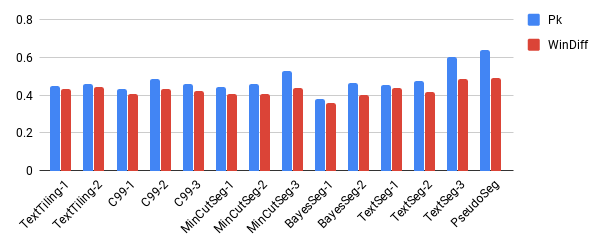
\includegraphics[width=.82\textwidth]{images/graficos/resumo-wd-pk.png}	
		% \label{fig:resumo-wd-pka}
		% 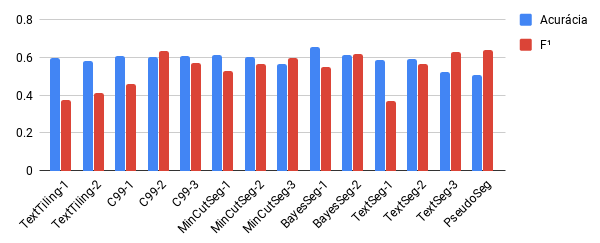
\includegraphics[width=.82\textwidth]{images/graficos/resumo-tradicionais.png}	
		% \label{fig:resumo-tradicionaisa}

	% \label{fig:resumo-segmentadores}
% \end{figure}



% \end{frame}


		\includegraphics[trim={ 0 235 0 16 },clip,page=1,width=0.73\textwidth]{images/distribuicao.pdf}
tela-principal-2-1.png
ficando os demais disponíveis para exploração pelo usuário.

Os tópicos mais similares à consulta ficam disponíveis para exploração.


Busca exploratória pelos tópicos mais similares à consulta.







O módulo de consulta aproveita a estrutura de dados interna para recuperar informações

Usa-se o modelo de espaço vetorial para ranquear os tópicos.








incorporar conhecimento de domínio aos dados












com isso é possivel identificar em cada ata

com isso é possível identificar trechos que tradam de um assunto
com isso é possível identificar os assuntos tratados em uma ata bem como sua 

com isso é possível identificar nas atas os trechos que tradam de um assunto


com isso é possível identificar os assuntos tratados em uma ata. 



Essa abordagem permite a expansão do espaço de busca além do conjunto de termos original de cada segmento, e a identificação de trechos mais relevantes à consulta.






\nblock{ Estrutura mais organizada} {
	\begin{itemize}
		\item  Segmentos agrupados por tópico.
		\item  Segmentos acrescidos de novos atributos (tópicos)
	\end{itemize}
}




\begin{center}
    \begin{minipage}{0.5\textwidth}
		\begin{description} \tiny
			\item[DT] Discordo Totalmente
			\item[DP] Discordo Parcialmente
			\item[NCND] Não Concordo Nem Discordo
			\item[CP] Concordo Parcialmente
			\item[CT] Concordo Totalmente
		\end{description}
    \end{minipage}
  \end{center}



\begin{center}
    \begin{minipage}{0.5\textwidth}
		\begin{description} \tiny
			\item[N] Nenhum
			\item[P] Poucos
			\item[NMNP] Nem Muitos nem Poucos
			\item[M] Muitos
			\item[T] Todos
		\end{description}
    \end{minipage}
  \end{center}



\begin{figure}[!h] \centering     %%% not \center
%	\subfigure{ \label{fig:kmeans}
		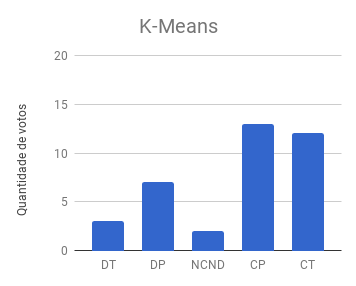
\includegraphics[width=.31\textwidth]{conteudo/capitulos/figs/figuras-experimento/Q1-KMeans.png}
%	}	
%	\subfigure{ \label{fig:lda}
		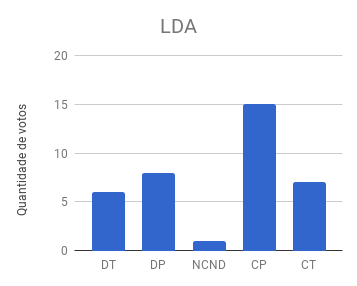
\includegraphics[width=.31\textwidth]{conteudo/capitulos/figs/figuras-experimento/Q1-LDA.png}
%	}
%	\subfigure{ \label{fig:plsa}
		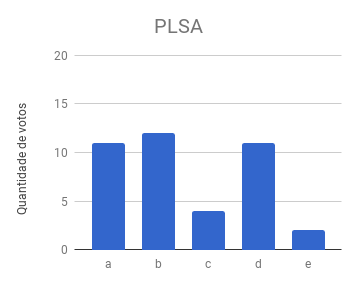
\includegraphics[width=.31\textwidth]{conteudo/capitulos/figs/figuras-experimento/Q1-PLSA.png}
%	} 
	\caption{Contagem de respostas referente a primeira questão cujo enunciado foi:\textit{``Todos os trechos apresentados compartilham um mesmo assunto.''}. O eixo vertical indica a frequência das alternativas representadas no eixo horizontal. }
	\label{fig:Q1}
\end{figure}












\begin{figure}[!h]
	\centering     %%% not \center

	\subfigure[a]{ \label{fig:a}
		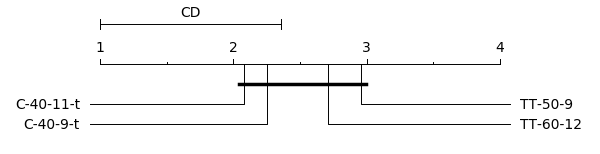
\includegraphics[width=70mm]{conteudo/capitulos/figs/CDs/WinDiff.png} }	
	\subfigure[b]{ \label{fig:b}
		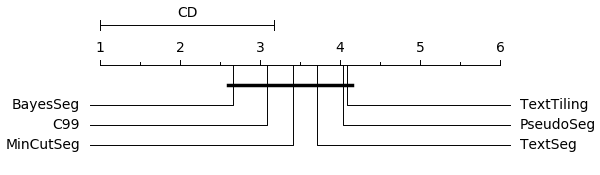
\includegraphics[width=70mm]{conteudo/capitulos/figs/CDs/Pk.png} }
	\subfigure[c]{ \label{fig:c}
		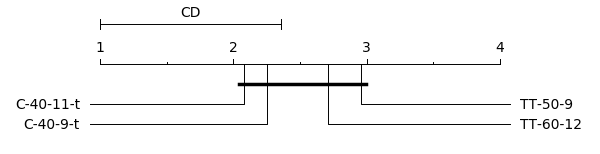
\includegraphics[width=70mm]{conteudo/capitulos/figs/CDs/Acuracy.png}}
	\subfigure[d]{ \label{fig:d}
		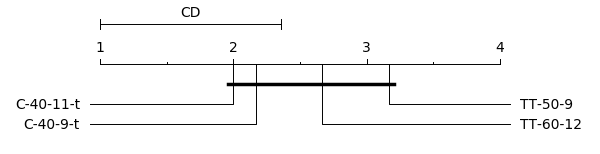
\includegraphics[width=75mm]{conteudo/capitulos/figs/CDs/Precision.png}}
	\subfigure[e]{ \label{fig:e}
		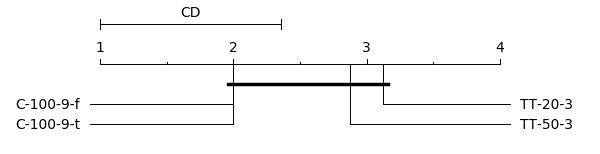
\includegraphics[width=70mm]{conteudo/capitulos/figs/CDs/Recall.png}}
	\subfigure[f]{ \label{fig:f}
		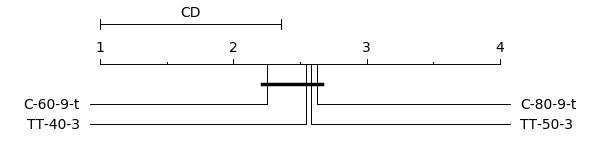
\includegraphics[width=70mm]{conteudo/capitulos/figs/CDs/F1.png}}

		\caption{Diagramas de Diferença Crítica sobre \textit{ranking} dos algoritmos de segmentação baseados em coesão léxica de acordo com valores de \textit{WindowDiff}, $P_k$, Acurácia, Precisão, Revocação e $F^1$.}
	\label{fig:CDs}
\end{figure}







  \begin{center}
	\begin{figure}[h!]

		\includegraphics[trim={ 0 235 0 0 },clip,page=1,width=\textwidth]{conteudo/capitulos/figs/doc-em-png/distribuicao.pdf}

	\end{figure}
\end{center}


\label{fig:distribuicao-ata}

\caption{Distribuição de tópicos em uma ata real. Cada tópico é representado por uma região colorida. Abaixo estão os descritores identificados pela cor do respectivo tópico. Os nomes de pessoas foram ocultados por não expressarem significado nesse trabalho.}





Informações contidas em grandes quantidades de texto;
Grandes volumes de texto com conteúdo irrelevante;
Documentos desestruturados;
Dificuldade em resgatar essas informações manualmente;


	\item Uma atas registra vários assuntos;

Motivação:
\begin{itemize}
	\item São fontes de consulta e utilizadas como referência e apoio a decisões; 
	\item Um assunto pode ser discutido diversas vezes em reuniões diferentes;
	\item É desejável recuperar um histórico dessas decisões ao longo do tempo;
	\item Necessidade de ferramentas automáticas;
\end{itemize}

Motivação:


Atas de reunião registram os assuntos tratados  como base de dados


\item Contém segmentos de texto com assuntos relativamente independentes; 



- Incapacidade humana em gerenciar grandes volumes de documentos;








Fiz um roteiro com:
Motivação
Objetivos
Proposta
Resultados
e Conclusão


acho que é esse roteiro mesmo
mas tipo
os "trabalhos relacionados"
meio que vão aparecer na motivação
pq vc vai falar que tem alguns estudos que segmentam determinados tipos de texto
mas não o que vc vai trabalhar lá em específico





hora que for explicar abordagem proposta
vc vai explicando cada etapa do seu framework
e lá vc vai mostrando a teoria envolvida com cada parte












A literatura apresenta abordagens 


Essa tarefa tem 2 passos principais:
\begin{itemize}
	\item Encontrar pontos onde há transição de assuntos;
	\item Identificar esse assunto;
\end{itemize}







Visão Geral 
imagem segmentação 
imagem documento com tópicos identificados nos segmentos



  % \begin{figure}[!h]
  % \centering
  % 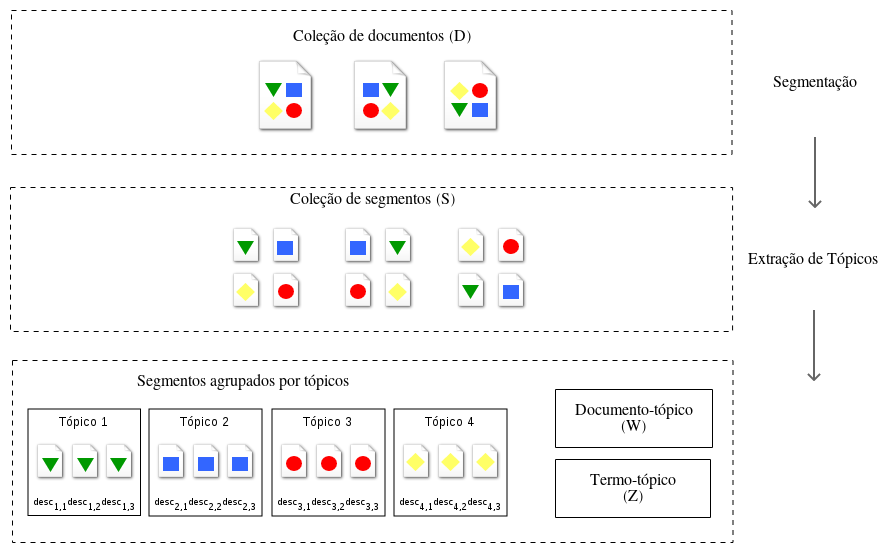
\includegraphics[width=.8\paperwidth]{images/estrutura.png}
  % \caption{Estrutura de dados interna e seu processo de geração.}
% %  \label{fig:#4}
  % \end{figure}





% \nblock{}{
\begin{itemize}
	\item Propor uma solução para identificar, organizar e consultar assuntos registrados em atas de reunião.  
	\item Utilizar técnicas de Segmentação textual em conjunto com modelos de Extração de Tópicos para:
		% \nblock{}{
			\begin{itemize}
	\item Gerar uma estrutura mais organizada que a coleção original.
	\item Utilizar a estrutura latente dos segmentos para Recuperação de Informação. 
		\end{itemize}
		% }
	% \item Dar início a investigação dessa abordagem no contexto de atas de reunião.
\end{itemize}
% }










o objetivo desse trabalho de mestrado é propor o 





desenvolvimento uma ferramenta 


para identificar, organizar e apresentar assuntos registrados em atas de reunião 


utilizando a estrutura latente de documentos segmentados em conjunto com técnicas de recuperação de informação.





% Propor uma solução para encontrar porções de texto relevantes à consulta.






\begin{figure}[!h] \centering     %%% not \center

%	\subfigure{ \label{fig:influencia-segRate-c99}
	  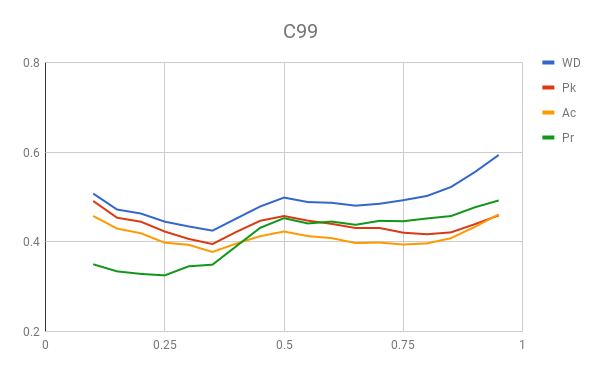
\includegraphics[width=.48\textwidth]{images/graficos/analiseNSegRate-C99.png}
%	}
%	\subfigure{ \label{fig:influencia-segRate-mc}
	  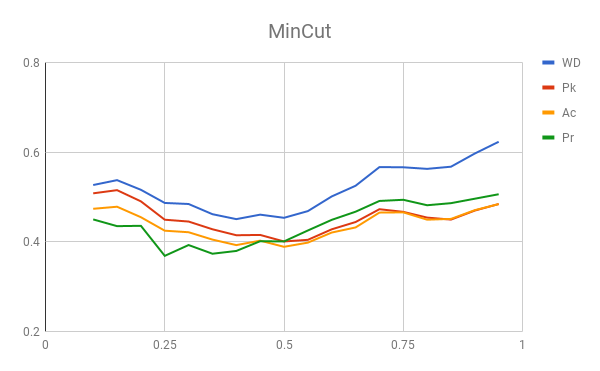
\includegraphics[width=.48\textwidth]{images/graficos/analiseNSegRate-MinCut.png}
%	}
%	\subfigure{ \label{fig:influencia-segRate-bs}
	  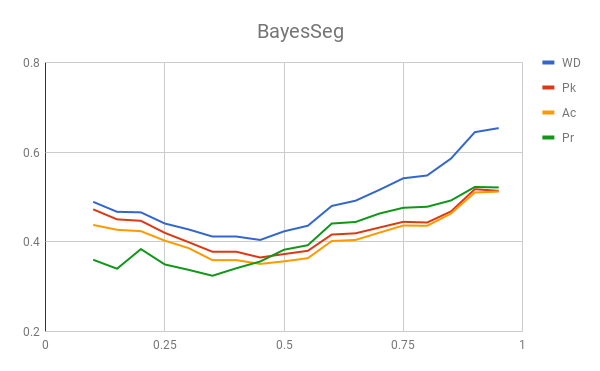
\includegraphics[width=.48\textwidth]{images/graficos/analiseNSegRate-Bayes.png}
%	}
%	\subfigure{ \label{fig:influencia-segRate-ui}
	  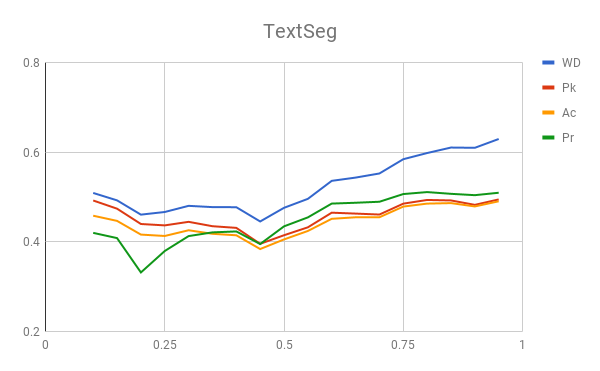
\includegraphics[width=.48\textwidth]{images/graficos/analiseNSegRate-UISeg.png}
%	}
	% \caption{Influência do taxa segmentos na eficiência dos algoritmos}
	\label{fig:influencia-SegRate}
\end{figure}





% Algoritmo & SR & WS & Step & W & RS & Prior & Disp. & LenCut\\

\begin{table}
\begin{tabular}{l | c | c | c | c }
Competitor Name & Swim & Cycle & Run & Total \\
\hline \hline
John T & 13:04 & 24:15 & 18:34 & 55:53 \\ 
Norman P & 8:00 & 22:45 & 23:02 & 53:47\\
Alex K & 14:00 & 28:00 & n/a & n/a\\
Sarah H & 9:22 & 21:10 & 24:03 & 54:35 
\end{tabular}
\caption{Triathlon results}
\end{table}





	\nblock{}{Algoritmos
		\begin{itemize}
			\item \textit{TextTiling};
			\item \textit{C99};
			\item \textit{BayesSeg};
			\item \textit{MinCut};
			\item \textit{TextSeg};
			\item \textit{PseudoSeg}.
		\end{itemize}
	}


	\nblock{}{Variação de Parâmetros
		\begin{itemize}
			\item WinSize (20-60), Step (30-55);
			\item W (sim/não), SR (.2-.7), RS (3-7);
			\item SR (auto, .3-.9), Prior (.08-.11), Disp (.1-.7);
			\item SR (.2-.7), LenCut (5-15);
			\item SR (auto, .1-.9),
			\item \textit{PseudoSeg}.
		\end{itemize}
	}


	% \nblock{}{Medidas
		% \begin{itemize}
		% \item Acurácia;
		% \item F$^1$;
		% \item WindowDiff;	
		% \item P$_k$.
		% \end{itemize}
	% }





